%\documentstyle[epsf,twocolumn]{jarticle}       %LaTeX2e仕様
\documentclass[twocolumn]{jarticle}     %pLaTeX2e仕様(platex.exeの場合)
% \documentclass[onecolumn]{ujarticle}   %pLaTeX2e仕様(uplatex.exeの場合)
%%%%%%%%%%%%%%%%%%%%%%%%%%%%%%%%%%%%%%%%%%%%%%%%%%%%%%%%%%%%%%
%%
%%  基本バージョン
%%
%%%%%%%%%%%%%%%%%%%%%%%%%%%%%%%%%%%%%%%%%%%%%%%%%%%%%%%%%%%%%%%%
\setlength{\topmargin}{-45pt}
%\setlength{\oddsidemargin}{0cm}
\setlength{\oddsidemargin}{-7.5mm}
%\setlength{\evensidemargin}{0cm}
\setlength{\textheight}{24.1cm}
%setlength{\textheight}{25cm}
\setlength{\textwidth}{17.4cm}
%\setlength{\textwidth}{172mm}
\setlength{\columnsep}{11mm}

%\kanjiskip=.07zw plus.5pt minus.5pt


% 【節が変わるごとに (1.1)(1.2) … (2.1)(2.2) と数式番号をつけるとき】
%\makeatletter
%\renewcommand{\theequation}{%
%\thesection.\arabic{equation}} %\@addtoreset{equation}{section}
%\makeatother

%\renewcommand{\arraystretch}{0.95} 行間の設定
%%%%%%%%%%%%%%%%%%%%%%%%%%%%%%%%%%%%%%%%%%%%%%%%%%%%%%%%
%\usepackage{graphicx}   %pLaTeX2e仕様(\documentstyle ->\documentclass)
\usepackage[dvipdfmx]{graphicx}
\usepackage{subcaption}
\usepackage{multirow}
\usepackage{amsmath}
\usepackage{url}
\usepackage{ulem}
\usepackage{algorithm}
\usepackage{algorithmic}
\usepackage{listings} %,jlisting} %日本語のコメントアウトをする場合jlistingが必要
%ここからソースコードの表示に関する設定
\lstset{
  basicstyle={\ttfamily},
  identifierstyle={\small},
  commentstyle={\smallitshape},
  keywordstyle={\small\bfseries},
  ndkeywordstyle={\small},
  stringstyle={\small\ttfamily},
  frame={tb},
  breaklines=true,
  columns=[l]{fullflexible},
  numbers=left,
  xrightmargin=0zw,
  xleftmargin=3zw,
  numberstyle={\scriptsize},
  stepnumber=1,
  numbersep=1zw,
  lineskip=-0.5ex
}
%%%%%%%%%%%%%%%%%%%%%%%%%%%%%%%%%%%%%%%%%%%%%%%%%%%%%%%%
\begin{document}

	%bibtex用の設定
	%\bibliographystyle{ujarticle}

	\twocolumn[
		\noindent
		\hspace{1em}
		2020 年 9 月 11 日
		ゼミ資料
		\hfill
		B4 杉山 竜弥
		\vspace{2mm}

		\hrule
		\begin{center}
			{\Large \bf 進捗報告}
		\end{center}
		\hrule
		\vspace{9mm}
	]

	% ‚ここから 文章 Start!
\section{今週やったこと}
\begin{itemize}
	\item VGGのアーキテクチャ探索の実装と実験
\end{itemize}

\section{問題設定}
DARTSの追実験が概ね成功したので, 新たにアーキテクチャの探索を設定してみることにした.
調査の結果, VGGの最適なショートカット位置をDARTSで探索することを問題に定めた.

図\ref{fig:connect}にショートカット位置の関係を示した.


\begin{figure}[tb]
	\begin{center}
		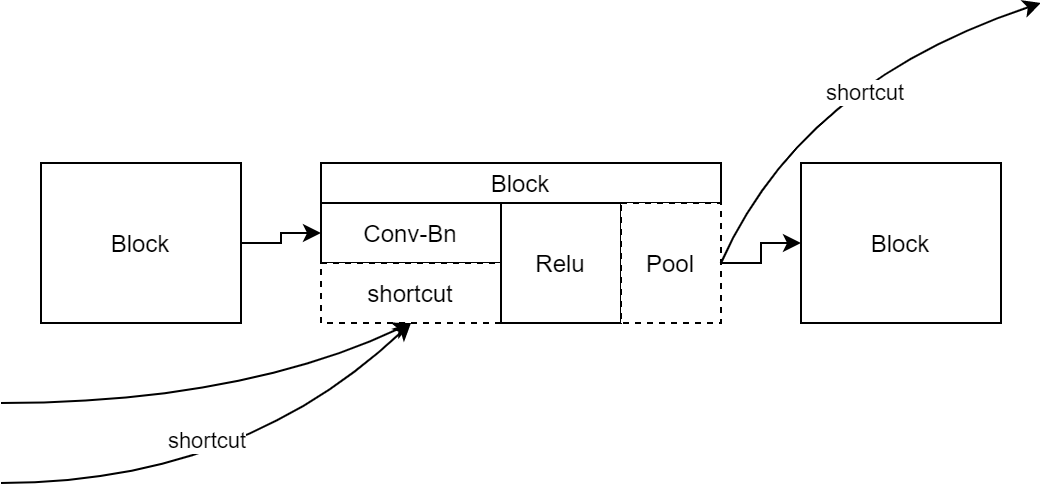
\includegraphics[clip,width=7.5cm]{connect.png}
		\caption{ショートカット位置}
		\label{fig:connect}
	\end{center}
\end{figure}

\section{実験}

ショートカット部分は
\begin{equation}
  \label{equ:cut}
  x_i = {\rm ConvBn}_{i}(x_{i-1}) + \sum_j \alpha_{ij} * {\rm shortcut}_{ij} (x_j)
\end{equation}
のように, concatではなくショートカットの加重和との和とした.

表\ref{tab:setting}に実験設定を示した.
もととなるモデルはVGG11とした.
したがってBlock数は8となった.
このBlockに対して可能な接続の組み合わせを全て探索することにした.

今回はアーキテクチャ探索($\alpha$を得る)段階までを行い, 性能は評価していない.

\begin{table}[tb]
  \begin{center}
    \caption{実験の設定}
    \begin{tabular}{|c|c|} \hline
      model & VGG11 \\ \hline
      Optim(model) & SGD(lr=0.01, momentum=0.9) \\ \hline
      Optim($\alpha$) & Adam(lr=0.005, $\beta$=(0.5, 0.999)) \\ \hline
      Loss & Cross Entropy Loss \\ \hline
      dataset & cifar10 \\ \hline
      batch size & 64 \\ \hline
      train data & 25000 + 25000 \\ \hline
      epoch & 100 \\ \hline
    \end{tabular}
    \label{tab:setting}
  \end{center}
\end{table}

\section{結果}

図\ref{fig:acc}には訓練とテストの精度を示した.
テスト精度は最大で85.54\%であった.

表\ref{tab:alpha_max}, \ref{tab:alpha}にはアーキテクチャー探索結果の$\alpha$の重みを示した.
表\ref{tab:alpha}が生の値で, (\ref{equ:cut})式ではsoftmaxした表\ref{tab:alpha_max}の値を用いている. 表中の0.00となっている場所はショートカットが存在しない.

\begin{figure}[tb]
	\begin{center}
		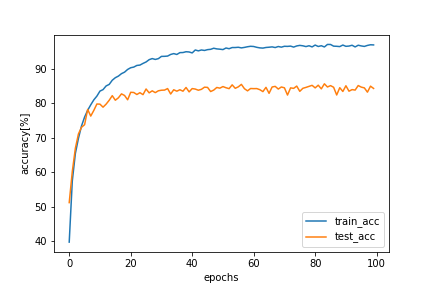
\includegraphics[clip,width=7.5cm]{acc.png}
		\caption{精度}
		\label{fig:acc}
	\end{center}
\end{figure}
% \begin{figure}[tb]
% 	\begin{center}
% 		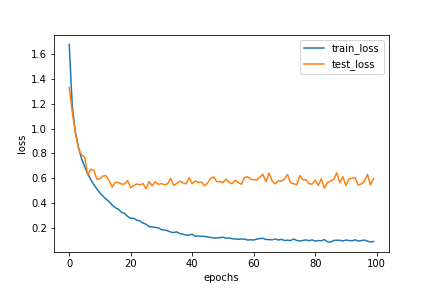
\includegraphics[clip,width=7.5cm]{loss.png}
% 		\caption{損失}
% 		\label{fig:loss}
% 	\end{center}
% \end{figure}

\begin{table*}[tb]
  \begin{center}
    \caption{$\alpha$の重み (softmax)}
    \begin{tabular}{|c|c|c|c|c|c|c|c|c|} \hline
      i \verb|\| j & 1 & 2 & 3 & 4 & 5 & 6 \\ \hline
      1 & 0.0000 & 0.0000 & 0.0000 & 0.0000 & 0.0000 & 0.0000 \\ \hline
      2 & 0.0000 & 0.0000 & 0.0000 & 0.0000 & 0.0000 & 0.0000 \\ \hline
      3 & 1.0000 & 0.0000 & 0.0000 & 0.0000 & 0.0000 & 0.0000 \\ \hline
      4 & 0.2019 & 0.7981 & 0.0000 & 0.0000 & 0.0000 & 0.0000 \\ \hline
      5 & 0.2144 & 0.1256 & 0.6600 & 0.0000 & 0.0000 & 0.0000 \\ \hline
      6 & 0.0588 & 0.8246 & 0.0570 & 0.0596 & 0.0000 & 0.0000 \\ \hline
      7 & 0.0368 & 0.8497 & 0.0374 & 0.0386 & 0.0375 & 0.0000 \\ \hline
      8 & 0.1238 & 0.1484 & 0.2058 & 0.2357 & 0.2417 & 0.0446 \\ \hline
    \end{tabular}
    \label{tab:alpha_max}
  \end{center}
\end{table*}

\begin{table*}[tb]
  \begin{center}
    \caption{$\alpha$の重み}
    \begin{tabular}{|c|c|c|c|c|c|c|c|c|} \hline
      i \verb|\| j & 1 & 2 & 3 & 4 & 5 & 6 \\ \hline
      1 & 0.0000 & 0.0000 & 0.0000 & 0.0000 & 0.0000 & 0.0000 \\ \hline
      2 & 0.0000 & 0.0000 & 0.0000 & 0.0000 & 0.0000 & 0.0000 \\ \hline
      3 & 0.0000 & 0.0000 & 0.0000 & 0.0000 & 0.0000 & 0.0000 \\ \hline
      4 & -0.6871 & 0.6871 & 0.0000 & 0.0000 & 0.0000 & 0.0000 \\ \hline
      5 & -0.1982 & -0.7329 & 0.9261 & 0.0000 & 0.0000 & 0.0000 \\ \hline
      6 & -0.6557 & 1.9855 & -0.6870 & -0.6411 & 0.0000 & 0.0000 \\ \hline
      7 & -0.6814 & 2.4581 & -0.6656 & -0.6325 & -0.6629 & 0.0000 \\ \hline
      8 & -0.1647 & 0.0171 & 0.3440 & 0.4793 & 0.5046 & -1.1853 \\ \hline
    \end{tabular}
    \label{tab:alpha}
  \end{center}
\end{table*}

\section{考察}

VGGに対してショートカットの重みを学習できることを確認した.
探索空間を自分で設計してみて分った, DARTSの難しいところ.
\begin{itemize}
  \item 微分できるように候補を同時に組み込む必要がある
  \item $\alpha$からアーキテクチャを決定する必要がある
\end{itemize}

\section{今後の予定}
% なんとなくなんかの勉強をするとかではなく具体的に

DARTSは得られた重みに対して, 適切なアーキテクチャを決定する必要がある.
決定する方法はいくつか考えられるため, 次回はそれぞれの手法の性能を比較したい.
図\ref{fig:result}には必ず1つの接続を持つことを仮定した場合のVGGの構造を示した.

\begin{figure*}[tb]
	\begin{center}
		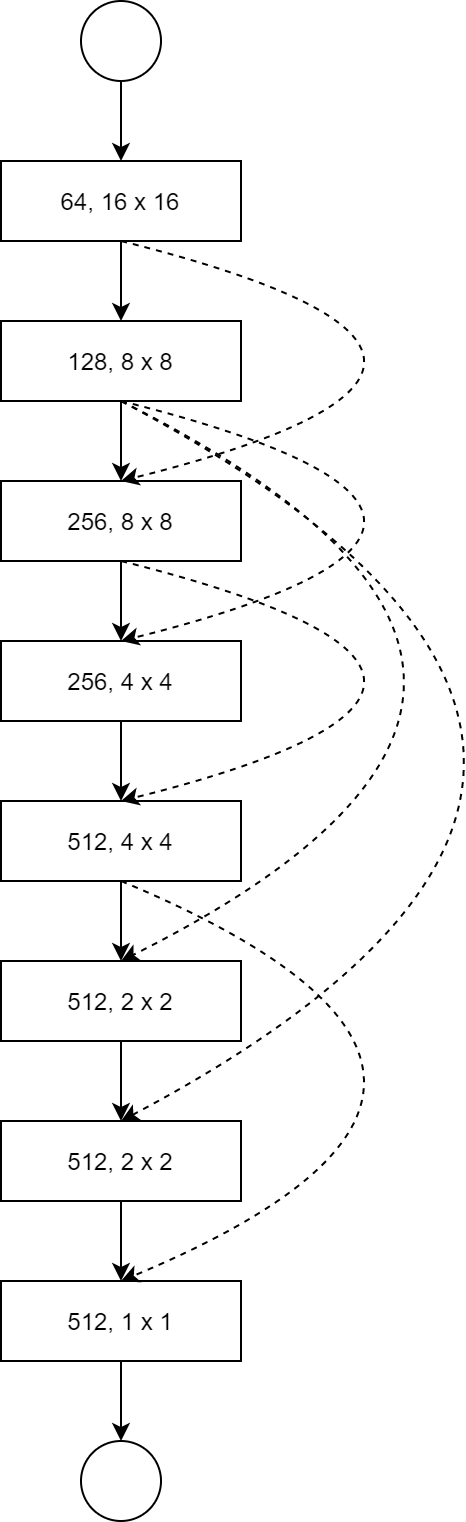
\includegraphics[clip,width=5.5cm]{result.png}
		\caption{接続を仮定したモデル}
		\label{fig:result}
	\end{center}
\end{figure*}

% \begin{itemize}
%   \item アーキテクチャの性能評価
% \end{itemize}

\section{ソースコード}
% 埋め込みでもGitでもいいので参照できるように
Githubの同階層を参照.

% 参考文献リスト
\bibliographystyle{unsrt}
\bibliography{ref}
\end{document}
